\documentclass{beamer}
\usepackage[utf8]{inputenc}

\usetheme{Madrid}
\usecolortheme{default}
\usepackage{amsmath,amssymb,amsfonts,amsthm}
\usepackage{txfonts}
\usepackage{tkz-euclide}
\usepackage{listings}
\usepackage{adjustbox}
\usepackage{array}
\usepackage{tabularx}
\usepackage{gvv}
\usepackage{lmodern}
\usepackage{circuitikz}
\usepackage{tikz}
\usepackage{graphicx}

\setbeamertemplate{page number in head/foot}[totalframenumber]

\usepackage{tcolorbox}
\tcbuselibrary{minted,breakable,xparse,skins}



\definecolor{bg}{gray}{0.95}
\DeclareTCBListing{mintedbox}{O{}m!O{}}{%
  breakable=true,
  listing engine=minted,
  listing only,
  minted language=#2,
  minted style=default,
  minted options={%
    linenos,
    gobble=0,
    breaklines=true,
    breakafter=,,
    fontsize=\small,
    numbersep=8pt,
    #1},
  boxsep=0pt,
  left skip=0pt,
  right skip=0pt,
  left=25pt,
  right=0pt,
  top=3pt,
  bottom=3pt,
  arc=5pt,
  leftrule=0pt,
  rightrule=0pt,
  bottomrule=2pt,
  toprule=2pt,
  colback=bg,
  colframe=orange!70,
  enhanced,
  overlay={%
    \begin{tcbclipinterior}
    \fill[orange!20!white] (frame.south west) rectangle ([xshift=20pt]frame.north west);
    \end{tcbclipinterior}},
  #3,
}
\lstset{
    language=C,
    basicstyle=\ttfamily\small,
    keywordstyle=\color{blue},
    stringstyle=\color{orange},
    commentstyle=\color{green!60!black},
    numbers=left,
    numberstyle=\tiny\color{gray},
    breaklines=true,
    showstringspaces=false,
}
\begin{document}

\title 
{1.9.22}
\date{August 25,2025}


\author 
{Kavin B-EE25BTECH11033}






\frame{\titlepage}
\begin{frame}{Question}
Find the value of $y$ for which the distance between the points $\vec{P}(2,-3)$ and $\vec{Q}(10,y)$ is $10$ units.
\end{frame}



\begin{frame}{Theoretical Solution}

Given the points,
\begin{align}
    \vec{P}=\begin{myvec}{2\\-3}\end{myvec}\ \ 
    \vec{Q}=\begin{myvec}{10\\y}\end{myvec}
\end{align}
The distance between the points \vec{P} and \vec{Q} is given as,
\begin{align}
d = \norm{\vec{P}-\vec{Q}} = 10
\end{align}
\end{frame}

\begin{frame}{Formulae}
\textbf{The length of a vector  is  defined as}
\begin{align}
\label{eq:side-length}
	\norm{\vec{P}-\vec{Q}} \triangleq \sqrt{(\vec{P}-\vec{Q})^{\top}(\vec{P}-\vec{Q})}
\end{align}
\end{frame}


\begin{frame}{Theoretical Solution}
\begin{align}
            (\vec{P}-\vec{Q})^\top (\vec{P}-\vec{Q}) = \norm{\vec{P}-\vec{Q}}^2\\
            (\vec{P}-\vec{Q})^\top (\vec{P}-\vec{Q}) = 10^2\\
\because
		\vec{P} - \vec{Q} = \myvec{2\\-3} - \myvec{10\\y} &= \myvec{-8\\-3-y},\\
        \implies\myvec{-8\\-3-y}^\top\myvec{-8\\-3-y} &= 10^2
\end{align}

\end{frame}

\begin{frame}{Theoretical Solution}

\begin{align}
         \implies\myvec{-8 & -3-y}\myvec{-8\\-3-y} &= 100\\
        \implies 8^2 + (3+y)^2 = 100\\
        \implies (3+y)^2=36\\
        \implies 3+y=\pm6\\
        \implies y=3, -9
\end{align}
\bigskip
Therefore the points $\brak{10,3}$ and $\brak{10,-9}$ are at a distance of $10$ units from the point \vec{P}.
\end{frame}


\begin{frame}[fragile]
    \frametitle{C Code - A function to find the y coordinates of Q}

    \begin{lstlisting}

#include <stdio.h>
#include <math.h>

int findYCoordinates(double px, double py, double qx, double d, double *y1, double *y2) {
    double term = pow(d, 2) - pow(qx - px, 2);
    double sqrt_term = sqrt(term);
    *y1 = py + sqrt_term;
    *y2 = py - sqrt_term;
    
    return 1; 
}
    \end{lstlisting}
\end{frame}

\begin{frame}[fragile]
    \frametitle{Python Code}
    \begin{lstlisting}
import numpy as np
import matplotlib.pyplot as plt
import ctypes
import os

c_lib=ctypes.CDLL('./code.so')

# --- 2. Define the C Function Signature in Python ---
# Get a handle to the C function
find_y_coordinates = c_lib.findYCoordinates

    \end{lstlisting}
\end{frame}

\begin{frame}[fragile]
    \frametitle{Python Code}
    \begin{lstlisting}
# Define the argument types (argtypes) for the C function
# double, double, double, double, *double, *double
find_y_coordinates.argtypes = [
    ctypes.c_double, ctypes.c_double,
    ctypes.c_double, ctypes.c_double,
    ctypes.POINTER(ctypes.c_double),
    ctypes.POINTER(ctypes.c_double)
]
# Define the return type (restype)
find_y_coordinates.restype = ctypes.c_int

    \end{lstlisting}
\end{frame}

\begin{frame}[fragile]
    \frametitle{Python Code}
    \begin{lstlisting}
# --- Prepare Inputs and Call the C Function ---
# Problem parameters
px, py = 2.0, -3.0
qx = 10.0
distance = 10.0

# Create C-compatible variables to hold the results (y1 and y2)
y1_c = ctypes.c_double()
y2_c = ctypes.c_double()

# Call the C function. Use ctypes.byref() to pass the variables by reference.
success = find_y_coordinates(px, py, qx, distance, ctypes.byref(y1_c), ctypes.byref(y2_c))


    \end{lstlisting}
\end{frame}

\begin{frame}[fragile]
    \frametitle{Python Code}
    \begin{lstlisting}
if not success:
    print("C function failed to find real coordinates. Check your inputs.")
    exit()

# Extract the Python values from the C-type objects
y1 = y1_c.value
y2 = y2_c.value

print(f"Values calculated by C function: y1 = {y1}, y2 = {y2}")
# --- Plot the Results ---
# Define the points using the values from the C function
P = np.array([px, py]).reshape(-1, 1)
Q1 = np.array([qx, y1]).reshape(-1, 1) # Use y1 from C
Q2 = np.array([qx, y2]).reshape(-1, 1) # Use y2 from C

    \end{lstlisting}
\end{frame}
\begin{frame}[fragile]
    \frametitle{Python Code}
    \begin{lstlisting}
# Plotting the lines from P to Q1 and P to Q2
plt.plot([P[0,0], Q1[0,0]], [P[1,0], Q1[1,0]], label=f'$PQ_1$ (distance={distance})')
plt.plot([P[0,0], Q2[0,0]], [P[1,0], Q2[1,0]], label=f'$PQ_2$ (distance={distance})')

# Combining all points for easy plotting and labeling
coords = np.block([[P, Q1, Q2]])
plt.scatter(coords[0, :], coords[1, :], color='red', zorder=5)
# Adding labels for each point
vert_labels = ['P', 'Q₁', 'Q₂']
for i, txt in enumerate(vert_labels):
    plt.annotate(f'{txt}\n({coords[0, i]:.0f}, {coords[1, i]:.0f})',
                 (coords[0, i], coords[1, i]),
                 textcoords="offset points",
                 xytext=(0, 10),
                 ha='center')
    \end{lstlisting}
\end{frame}
\begin{frame}[fragile]
    \frametitle{Python Code}
    \begin{lstlisting}
# --- Plot Formatting ---
ax = plt.gca()
ax.spines['top'].set_color('none')
ax.spines['left'].set_position('zero')
ax.spines['right'].set_color('none')
ax.spines['bottom'].set_position('zero')

plt.legend(loc='best')
plt.grid(True)
plt.axis('equal')
plt.title("Plot generated using values from C function")
# Save the plot to a file
plt.savefig('../figs/fig.png')


plt.show()

    \end{lstlisting}
\end{frame}


\begin{frame}{Plot}
    \centering
    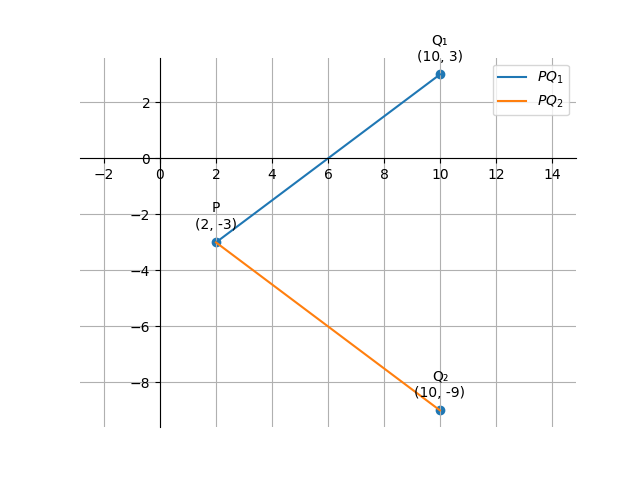
\includegraphics[width=\columnwidth, height=0.8\textheight, keepaspectratio]{figs/fig.png}     
\end{frame}


\end{document}